\documentclass[class=report, crop=false]{standalone}
\usepackage[subpreambles=true]{standalone}
\usepackage{import}
%%\usepackage{booktabs}
%\usepackage{tikz}

%\usepackage[utf8]{inputenc}
\usepackage[subpreambles=true]{standalone}
\usepackage{import}
\usepackage{pgfplots}
\pgfplotsset{compat=newest}
\usepgfplotslibrary{groupplots}
\usepgfplotslibrary{dateplot}
\usepackage{caption}
\usepackage{subcaption}
\usepackage{graphicx}
\usepackage{amsmath}
\usepackage{amssymb}
\usepackage[parfill]{parskip}
\usepackage{float}

% \usepackage{pgfplots}
% \usetikzlibrary{pgfplots.groupplots}
% \pgfplotsset{compat=1.9,height=0.3\textheight,legend cell align=left,tick scale binop=\times}
% \pgfplotsset{grid style={loosely dotted,color=darkgray!30!gray,line width=0.6pt},tick style={black,thin}}
% \pgfplotsset{every axis plot/.append style={line width=0.8pt}}
%
% \usepgfplotslibrary{external}
% % Für die Verwendung von 'external' müssen die folgenden Anpassungen in Abhängigkeit der
% % LaTeX Distribution durchgeführt werden:
%
% % fuer Texlive: pdflatex.exe -shell-escape -synctex=1 -interaction=nonstopmode %.tex
% \tikzexternalize[shell escape=-shell-escape]   % fuer TeXLive
%
% % fuer MikTeX:  pdflatex.exe -enable-write18 -synctex=1 -interaction=nonstopmode %.tex
% %\tikzexternalize[shell escape=-enable-write18] % fuer MikTex
%
%
%
% \tikzsetexternalprefix{graphics/pgfplots/} % Ordner muss ev. zuerst haendisch erstellt werden


\begin{document}

\subsection{Custom Kalman Filter}\label{subsec:customkalman}
State estimation is an important part of any mobile robot. Its accuracy can be refined by multiple sensors. In order to deal with sensor noise and other inaccuracies during our position estimation, we used a linear quadratic estimator known as the Kalman Filter.

It is widely used in control theory and control systems engineering. Its applications include aircraft, spacecraft, ships and robot motion planning.

\subsubsection{Kalman Filter Theory}\label{subsubsec:kalmanfilter}

The Kalman Filter is a recursive digital filter that uses the system's dynamic model with uncertainties and noisy sensor measurements to estimate the system state while minimizing errors.

It uses a relative weight called the Kalman gain that is used with the current state estimation and sensor measurements. Its purpose is to "trust" values more that have a smaller uncertainty and thus give a more reliable estimation. It achieves that by the using covariances of the measurements and known, also to some extent unknown, noise that effect the states.

The following system model seen in \eqref{eq:generickalman} is a generic model of the Kalman Filter we used. It is based on a lecture script from Kemmetm{\"u}ller, W and Kugi, A\cite{regelungssysteme1} that is currently used in the Automation Master degree course Control Systems 1 at TU Vienna.

\begin{equation}
\begin{gathered}
  \textbf{x}_{k+1} =
  \boldsymbol{\Phi}_k
  \textbf{x}_k +
  \boldsymbol{\Gamma}_k
  \textbf{u}_k +
  \textbf{G}_k
  \textbf{w}_k \\
  \textbf{y}_k =
  \textbf{C}_k
  \textbf{x}_k +
  \textbf{D}_k
  \textbf{u}_k +
  \textbf{H}_k
  \textbf{w}_k +
  \textbf{v}_k \\
  \textbf{x}(0) = \textbf{x}_0 \\
\end{gathered}\label{eq:generickalman}
\end{equation}

The system consists of a state vector $ \textbf{x}_k  \in  \mathbb{R}^n $, an input vector $ \textbf{u}_k \in \mathbb{R}^p $, an output(measurement) vector $ \textbf{y}_k \in \mathbb{R}^q $, a process noise vector $ \textbf{w}_k \in \mathbb{R}^r $, a measurement noise vector $ \textbf{v}_k \in \mathbb{R}^q $ and a time variant dynamic coefficient matrix $ \boldsymbol{\Phi}_k \in \mathbb{R}^{n \times n}$,
an input coupling matrix $ \boldsymbol{\Gamma}_k \in \mathbb{R}^{n \times p}$, a process noise input coupling matrix $ \boldsymbol{G}_k \in \mathbb{R}^{n \times r} $, a measurement sensitivity matrix $ \boldsymbol{C}_k \in \mathbb{R}^{q \times n} $, a measurement output coupling matrix $ \boldsymbol{D}_k \in \mathbb{R}^{q \times p}$ and a process noise output coupling matrix $ \textbf{H}_k \in \mathbb{R}^{q \times r} $.

\noindent
The following assumptions about the system were made:

\noindent
1. For the system noise vector $ \textbf{w}_k$ and measurement noise vector $ \textbf{v}_k $:
\begin{align*}
    E(\textbf{w}_k \textbf{w}_j^T) &= \textbf{R}_k \delta_{kj} & \textbf{R}_k &\ge \textbf{0} & E(\textbf{w}_k) &= \textbf{0} \\
    E(\textbf{v}_k \textbf{v}_j^T) &= \textbf{Q}_k \delta_{kj} & \textbf{Q}_k &\ge \textbf{0} & E(\textbf{v}_k) &= \textbf{0} \\
    E(\textbf{w}_k \textbf{v}_j^T) &= \textbf{0} & \textbf{H}_k  \textbf{Q}_k \textbf{H}_k^T &> \textbf{0}\\
\end{align*}\label{eq:assumption1}
Where $ \textbf{Q}_k \in \mathbb{R}^{r \times r} $ is the process noise covariance matrix and $ \textbf{R}_k \in \mathbb{R}^{q \times q} $ is the measurement noise covariance matrix and $ \delta_{kj} $ the Kroneckersymbol, which is $ \delta_{kj} = 1$ for $ k = j $ and $ \delta_{kj} = 0$ for $ k \neq j $.

\vspace{0.5cm}
\noindent
2. The expected value of the initial state vector $ \textbf{x}_0 $ and the initial state error covariance matrix $ \textbf{P}_0 $:
\begin{align*}
    E(\textbf{x}_0) &= \textbf{m}_0 & E([\textbf{x}_0 - \hat{\textbf{x}}_0][\textbf{x}_0 - \hat{\textbf{x}}_0]^T) &= \textbf{P}_0 \ge 0
\end{align*}\label{eq:assumption2}
Where $ \hat{\textbf{x}}_0 $ is a guess for the initial state vector $ \textbf{x}_0 $.

\noindent
3. The process noise vector $\textbf{w}_k$ and measurement noise vector $\textbf{v}_k$ are not correlated with the intial state vector $ \textbf{x}_0 $:
\begin{align*}
    E(\textbf{w}_k \textbf{x}_0^T) &= \textbf{0}\\
    E(\textbf{v}_k \textbf{x}_0^T)&= \textbf{0}\\
\end{align*}\label{eq:assumption3}
We modeled our system with the 7-dimensional state vector:

\begin{center}
 $\textbf{x}_k =
  \begin{bmatrix}
   x_k    \\
   y_k    \\
   v_k    \\
   a_k    \\
   \Psi_k \\
   \dot{\Psi}_k\\
   \ddot{\Psi}_k\\
  \end{bmatrix}
 $
\end{center}

where $x_k$ is the distance traveled in x, $y_k$ the distance traveled in y, $v_k$ is the robot's relative x speed, $a_k$ is the robot's relative x acceleration, $\Psi_k$ is the yaw of the robot, $\dot{\Psi}_k$ is the yaw speed and $\ddot{\Psi}_k$ the yaw acceleration.

Our system input is a joystick controller, which we use to move our robot forward and backward by setting the voltage on the motors, which generate a force or torque that move our robot.

\begin{center}
$ \textbf{u}_k =
\begin{bmatrix}
     \vartheta_k \\
     \eta_k    \\
 \end{bmatrix}
$
\end{center}

Where $\vartheta_k \in [-1,1]$ is our forwards and backwards signal and $\eta_k \in [-1,1]$ is our rotation signal in the right and left direction. The top force of the motors, by setting $\vartheta_k = \pm 1$, is the constant $\alpha$ and the top torque at $\eta_k = \pm 1$ is the constant $\beta$.

To construct our dynamic coefficient matrix $ \boldsymbol{\Phi_k} $ and input coupling matrix $ \boldsymbol{\Gamma_k} $, we used the following equations based on Newtonian kinematics, dynamics and Euler method:

\begin{align*}
    x_{k+1} &= x_k + v_k cos(\Psi_k) \Delta t + \frac{1}{2} a_k cos(\Psi_k) (\Delta t)^2 \\
    y_{k+1} &= y_k + v_k sin(\Psi_k) \Delta t + \frac{1}{2} a_k sin(\Psi_k) (\Delta t)^2 \\
    v_{k+1} &= v_k + a_k \Delta t\\
    m a_{k+1} &= \alpha \vartheta_k - \mu_v v_k\\
    \Psi_{k+1} &= \Psi_k + \Delta t \dot{\Psi}_{k} + \frac{1}{2} \ddot{\Psi}_k (\Delta t)^2 \\
    \dot{\Psi}_{k+1} &= \Psi_k + \Delta t \ddot{\Psi}_k \\
    J \ddot{\Psi}_{k+1} &= \beta \eta_k - \mu_{\dot{\Psi}_k} \dot{\Psi}_k\\
\end{align*}\label{eq:systemdyn}
The coefficients $m$ is the mass of the robot and $J$ is the moment of inertia(around the z-axis).

We modeled the moment of inertia $J$ as a rectangular block with the mass $m$(same as our robot), length $a$ and width $b$:
\begin{align*}
    J = \frac{m}{12} (a^2 + b^2)
\end{align*}

We furthermore reduced the number of parameters with $\alpha = b \beta$ in which we assume that the force from the motors is in $b/2$ from the center of rotation.

Our model of $J$ and $\beta$ is very simplistic and could be improved with proper modeling of parts and simulations, but since we are correcting this with our gyroscope, we can set an appropriate process noise $\textbf{Q}_k$ that reflects this modeling.

We assume that the drag is approximately proportional to the appropriate speed and the $\mu_v$ and $\mu_{\dot{\Psi}_k}$ are the linear drag coefficients.

Our system output $y_k$ is measured by our gyroscope and accelerometer in the IMU:
\begin{center}
 $ \textbf{y}_k =
  \begin{bmatrix}
   \zeta_k \\
   \chi_k  \\
  \end{bmatrix}
 $
\end{center}

where $\zeta_k$ is the acceleration measured in the x direction and $\chi_k$ is the measured yaw speed.

For our measurement matrix and our measurement output coupling matrix we used the following equations:
\begin{align*}
\zeta_k &= a_k\\
\chi_k &= \dot{\Psi}_{k}\\
\end{align*}\label{eq:outdyn}
Since we don't know the noise added to the system by our $\textbf{u}_k$ control input vector, we modeled it as an unknown system noise vector $\textbf{w}_k$ with a set standard deviation $\sigma$. The measurement noise vector $v_k$ was modeled similarly:

\begin{align*}
 \textbf{w}_k & = \begin{bmatrix}
  \sigma^{\vartheta_k}_k \\
  \sigma^{\eta_k}_k      \\
 \end{bmatrix} & \textbf{Q}_k & = \begin{bmatrix}
  (\sigma^{\vartheta_k}_k)^2 & 0                     \\
  0                          & (\sigma^{\eta_k}_k)^2 \\
 \end{bmatrix} \\
 \textbf{v}_k & = \begin{bmatrix}
  \sigma^{\zeta_k}_k \\
  \sigma^{\chi_k}_k  \\
 \end{bmatrix} & \textbf{R}_k & = \begin{bmatrix}
  (\sigma^{\zeta_k}_k)^2 & 0                     \\
  0                      & (\sigma^{\chi_k}_k)^2 \\
 \end{bmatrix} \\
\end{align*}\label{eq:noisemodel}
Putting together all of the previous equations into the form \eqref{eq:generickalman} we get:
\begin{gather*}
    \begin{bmatrix}
     \hat{x}_{k+1}^-    \\
     \hat{y}_{k+1}^-    \\
     \hat{v}_{k+1}^-    \\
     \hat{a}_{k+1}^-    \\
     \hat{\Psi}_{k+1}^- \\
     \hat{\dot{\Psi}}_{k+1}^- \\
     \hat{\ddot{\Psi}}_{k+1}^- \\
    \end{bmatrix} =
    \boldsymbol{\Phi}_k
    \begin{bmatrix}
     \hat{x}_{k}^+    \\
     \hat{y}_{k}^+    \\
     \hat{v}_{k}^+    \\
     \hat{a}_{k}^+    \\
     \hat{\Psi}_{k}^+ \\
     \hat{\dot{\Psi}}_{k}^+\\
     \hat{\ddot{\Psi}}_{k}^+\\
    \end{bmatrix} +
    \boldsymbol{\Gamma}_k
    \begin{bmatrix}
     \vartheta_k \\
     \eta_k      \\
    \end{bmatrix} +
    \textbf{G}_k
    \begin{bmatrix}
     \sigma^{\vartheta_k}_k \\
     \sigma^{\eta_k}_k      \\
    \end{bmatrix}\\
    \begin{bmatrix}
     \zeta_k \\
     \chi_k  \\
    \end{bmatrix} =
    \textbf{C}_k
    \begin{bmatrix}
     \hat{x}_{k}^- \\
     \hat{y}_{k}^- \\
     \hat{v}_{k}^- \\
     \hat{a}_{k}^- \\
     \Psi_{k}^-    \\
     \dot{\Psi}_{k}^- \\
     \ddot{\Psi}_{k}^- \\
    \end{bmatrix} +
    \textbf{D}_k
    \begin{bmatrix}
     \vartheta_k \\
     \eta_k      \\
    \end{bmatrix} +
    \textbf{H}_k
    \begin{bmatrix}
     \sigma^{\vartheta}_k \\
     \sigma^{\eta}_k      \\
    \end{bmatrix} +
    \begin{bmatrix}
     \sigma^{\zeta_k}_k \\
     \sigma^{\chi_k}_k  \\
    \end{bmatrix} \\
\end{gather*}

with:

\begin{gather*}
    \boldsymbol{\Phi}_k = \begin{bmatrix}
     1 & 0 &  cos(\hat{\Psi}_{k}^+) \Delta t & \frac{1}{2} cos(\hat{\Psi}_{k}^+) (\Delta t)^2  & 0 & 0 & 0\\
     0 & 1 &  sin(\hat{\Psi}_{k}^+) \Delta t & \frac{1}{2} sin(\hat{\Psi}_{k}^+) (\Delta t)^2 & 0 & 0 & 0\\
     0 & 0 & 1                              & \Delta t & 0 & 0 & 0\\
     0 & 0 & - \mu_{v} / m           & 0 & 0 & 0 & 0\\
     0 & 0 & 0 & 0                          & 1 & \Delta t & \frac{1}{2} (\Delta t)^2\\
     0 & 0 & 0 & 0 & 0 & 1 & \Delta t\\
     0 & 0 & 0 & 0 & 0 & - \mu_{\dot{\Psi}} / J & 0\\
    \end{bmatrix} \\
    \boldsymbol{\Gamma}_k =
    \begin{bmatrix}
     0      & 0             \\
     0      & 0             \\
     0      & 0             \\
     \alpha / m & 0             \\
     0      & 0 \\
     0      & 0             \\
     0      & \beta / J \\
    \end{bmatrix},
    \textbf{G}_k = \begin{bmatrix}
     0      & 0             \\
     0      & 0             \\
     0      & 0             \\
     \alpha / m & 0             \\
     0      & 0 \\
     0      & 0             \\
     0      & \beta / J \\
    \end{bmatrix} \\
    \textbf{C}_k =
    \begin{bmatrix}
     0 & 0 & 0 & 1 & 0 & 0 & 0 \\
     0 & 0 & 0 & 0 & 0 & 1 & 0\\
    \end{bmatrix},
    \textbf{D}_k =
    \begin{bmatrix}
     0 & 0     \\
     0 & 0 \\
    \end{bmatrix},
    \textbf{H}_k =
    \begin{bmatrix}
     0 & 0 \\
     0 & 0 \\
    \end{bmatrix}
\end{gather*}\label{eqn:fullsystem}
where the vector $\hat{\textbf{x}}_k^-$ is an "a priori" state estimation, the vector $\hat{\textbf{x}}_k^+$ is an "a posteriori" state estimation, which is an output corrected estimation of the "a priori" state, and an extrapolated $\hat{\textbf{x}}_{k+1}^+$, which then becomes the next iteration's "a priori" state.

The process noise input coupling matrix $\textbf{G}_k$ is filled with zeros(except for the input dimensions) because the process noise in the current iteration was already included by the last one, therefore it should not impact the rest of our current states.

The process noise output coupling matrix $\textbf{H}_k$ was filled with zeros, because the process noise $\textbf{w}_k$ shouldn't impact our measurement $\textbf{y}_k$ since it is already included in $\hat{\textbf{x}}_{k}^-$ from the last iteration.

Now that our system was constructed, we set the initial state vector $\textbf{x}_0 = \textbf{0}$ and the state error estimation matrix $\textbf{P}_0 = \textbf{0}$ and executed the following steps:

\noindent
1, Calculate Kalman gain matrix:
\vspace{0.5cm}
\begin{center}
$ \hat{\textbf{L}}_k = \textbf{P}^-_k \textbf{C}^T_k (\textbf{C}_k \textbf{P}^-_k \textbf{C}^T_k + \textbf{H}_k \textbf{Q}_k \textbf{H}^T_k + \textbf{R}_k)^{-1} $
\end{center}
\vspace{0.5cm}
2, Update state vector:
\vspace{0.5cm}
\begin{center}
$ \hat{\textbf{x}}^+_k = \hat{\textbf{x}}^-_k + \hat{\textbf{L}}_k (\textbf{y}_k - \textbf{C}_k \hat{\textbf{x}}^-_k - \textbf{D}_k \textbf{u}_k) $
\end{center}
\vspace{0.5cm}
3, Update state error covariance matrix:
\vspace{0.5cm}
\begin{center}
$ \textbf{P}^+_k = (\textbf{E} - \hat{\textbf{L}}_k \textbf{C}_k ) \textbf{P}^-_k $
\end{center}
\vspace{0.5cm}
4, Extrapolate state vector:
\vspace{0.5cm}
\begin{center}
$ \hat{\textbf{x}}^-_{k+1} = \boldsymbol{\Phi}_k \textbf{x}^+_k + \boldsymbol{\Gamma}_k \textbf{u}_k $
\end{center}
\vspace{0.5cm}
5, Extrapolate state error covariance matrix:
\vspace{0.5cm}
\begin{center}
$ \textbf{P}^-_{k+1} = \boldsymbol{\Phi}_k \textbf{P}^+_k \boldsymbol{\Phi}^T_k + \textbf{G}_k \textbf{Q}_k \textbf{G}^T_k $
\end{center}

\vspace{0.5cm}

Steps 2 and 3 are the "a posteriori" estimations, which were used in all of the figures in the thesis unless stated otherwise.

\subsubsection{Kalman Filter with adaptive process noise}\label{subsubsec:kfapn}

Our model of the Kalman Filter doesn't account for the ramp-up time of the motors before they reach their desired actuation force once the voltage is applied on them.

In order to combat this, we adapt the state estimation by increasing our noise covariance matrix $\textbf{Q}_k$ during this delay.

We first introduce a ratio matrix $\boldsymbol{\Upsilon}_k$ that describes our process noise covariance matrix $\textbf{Q}_k$ in relation to the measurement noise covariance matrix $\textbf{R}_k$:
\begin{align*}
 \textbf{Q}_k              & =  \boldsymbol{\Upsilon}_k \textbf{R}_k &
 \begin{bmatrix}
  (\sigma^{\vartheta_k}_k)^2 & 0                     \\
  0                          & (\sigma^{\eta_k}_k)^2 \\
 \end{bmatrix} & =  \begin{bmatrix}
  (\varrho_{\vartheta\zeta})^2 & 0      \\
  0      & (\varrho_{\eta\chi})^2 \\
 \end{bmatrix}
 \begin{bmatrix}
  (\sigma^{\zeta_k}_k)^2 & 0                     \\
  0                      & (\sigma^{\chi_k}_k)^2 \\
 \end{bmatrix}
\end{align*}\label{eq:ratio}

To respond to the jumps from our joystick we used a moving weighted window with a set length N.

We implemented a mirrored sigmoid curve using the logistic function in our moving weighted window due its ability to hold the peak relatively high before it decreases rapidly closer to its half-life.

We calculate the $w_k$ weights of a moving weighted window of length $N$ as:
\begin{align*}
 \textbf{x}_k & = \left\{ x:x = \dfrac{n}{N}, n \in (0,N), n \in \mathbb{N} \right\}   \\
 \textbf{w}_k & = \dfrac{ 1 }{ 1 + e^{\alpha ( \textbf{x}_k - \frac{1}{2})} }
\end{align*}

\vspace{0.5cm}

\begin{figure}[H]
 \begin{center}
  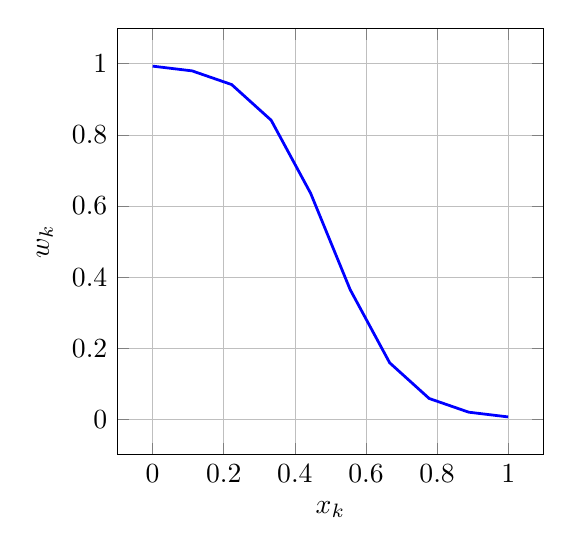
\begin{tikzpicture}[
    declare function={sig(\x) = 1 / (1 + exp(10*(\x - 0.5)));}
   ]
   \begin{axis}[
     unit vector ratio =1 1,
     domain=0:1,
     samples=10,
     yticklabel style={
       /pgf/number format/fixed,
       /pgf/number format/precision=5
      },
     width=7cm,
     height=7cm,
     xtick distance=0.2,
     ytick distance=0.2,
     xlabel={$x_k$},
     ylabel={$w_k$},
     grid=both,
     grid style={
       line width=.1pt,
       draw=gray!10},
     major grid style={
       line width=.2pt,
       draw=gray!50
      },
    ]
    \addplot [color=blue, mark=none,line width=1pt,mark size=1pt] {sig(x)};
   \end{axis}
  \end{tikzpicture}
\end{center}
 \caption{Moving Mirrored Sigmoid Weighted Window of $N=10$ and $\alpha=10$}\label{fig:sigwin}
\end{figure}

\vspace{0.5cm}

To track changes in the input vector $\textbf{u}_k$, we create a fixed $N$ length queue $\textbf{q}_k$ of $\Delta \textbf{u}_k$ elements, to which we enqueue $\Delta \textbf{u}_k =  \textbf{u}_k - \textbf{u}_{k-1}$ before every iteration and dequeue the first element.

In case of $\textbf{q}_k=0$ the process noise covariance matrix $\textbf{Q}_k$ shouldn't change, so we model it as:
\begin{align*}
    \textbf{Q}_k = \boldsymbol{\Upsilon}_k \textbf{R}_k (1+ \Delta \textbf{Q}_k) \\
\end{align*}
Where:
\begin{align*}
\Delta \textbf{Q}_k &=
\begin{bmatrix}
    \dfrac{M_1}{max(\textbf{q}_k^{\vartheta_k})} \sum_{i=1}^{N} q_{N+1-i}^{\vartheta_k} w_i & 0 \\
    0 & \dfrac{M_2}{max(\textbf{q}_k^{\eta_k})} \sum_{i=1}^{N} q_{N+1-i}^{\eta_k} w_i \\
\end{bmatrix}
\end{align*}

and $M_1, M_2 \in \mathbb{R}$ are constants for scaling the peak, $\textbf{q}_k^{\vartheta_k}, \textbf{q}_k^{\eta_k}$ are the queues corresponding to the elements of the input vector's $\Delta \textbf{u}_k$.

\subsubsection{Simulation}\label{subsubsec:sim}

In order to test our Kalman Filter, we first simulated an approximate v state of our robot where we drive it in a straight line with the help of a box function we used as an input.

Next we we create the differential of the v state to get the a state and add some noise to be used as a system output. This can be seen figure \ref{fig:vsim}.

The top speed of our robot was calculated with:
\begin{align*}
    \hat{v} &= \dfrac{\alpha \vartheta_k}{\mu_v}
\end{align*}

\vspace{0.5cm}

\begin{figure}[H]
\begin{flushleft}
  \begin{tikzpicture}
    \begin{axis}[
      yticklabel style={
        /pgf/number format/fixed,
        /pgf/number format/precision=5
      },
      width=12cm,
      height=5cm,
      ytick distance=0.2,
      xtick distance = 1,
      xlabel={Time $[s]$},
      ylabel={$ \textbf{u}^\vartheta_k$ $[m/s]$},
      grid=both,
      grid style={
        line width=.1pt,
        draw=gray!10},
        major grid style={
          line width=.2pt,
          draw=gray!50
        },
      ]
      \addplot+[color=blue, mark=none,line width=1pt,mark size=1pt] table {plots/line_sim0_u0.csv};
    \end{axis}
  \end{tikzpicture}
\end{flushleft}

\begin{flushleft}
  \begin{tikzpicture}
    \begin{axis}[
      yticklabel style={
        /pgf/number format/fixed,
        /pgf/number format/precision=5
      },
      width=12cm,
      height=5cm,
      ytick distance=0.2,
      xtick distance = 1,
      xlabel={Time $[s]$},
      ylabel={Simulated v state $[m/s] $},
      grid=both,
      grid style={
        line width=.1pt,
        draw=gray!10},
        major grid style={
          line width=.2pt,
          draw=gray!50
        },
      ]
      \addplot+[color=blue, mark=none,line width=1pt,mark size=1pt] table {plots/line_sim0_x2.csv};
    \end{axis}
  \end{tikzpicture}
\end{flushleft}
\begin{flushleft}
  \begin{tikzpicture}
    \begin{axis}[
      yticklabel style={
        /pgf/number format/fixed,
        /pgf/number format/precision=5
      },
      width=12cm,
      height=5cm,
      ytick distance=2.5,
      xtick distance = 1,
      xlabel={Time $[s]$},
      ylabel={Simulated a state $[m/s^2] $},
      grid=both,
      grid style={
        line width=.1pt,
        draw=gray!10},
        major grid style={
          line width=.2pt,
          draw=gray!50
        },
      ]
      \addplot+[color=blue, mark=none,line width=1pt,mark size=1pt] table {plots/line_sim0_x3.csv};
    \end{axis}
  \end{tikzpicture}
\end{flushleft}
\begin{flushleft}
  \begin{tikzpicture}
    \begin{axis}[
      yticklabel style={
        /pgf/number format/fixed,
        /pgf/number format/precision=5
      },
      width=12cm,
      height=5cm,
      ytick distance=2.5,
      xtick distance = 1,
      xlabel={Time $[s]$},
      ylabel={$ \textbf{y}^\zeta_k$ $[m/s^2] $},
      grid=both,
      grid style={
        line width=.1pt,
        draw=gray!10},
        major grid style={
          line width=.2pt,
          draw=gray!50
        },
      ]
      \addplot+[color=blue, mark=none,line width=1pt,mark size=1pt] table {plots/line_sim0_y0.csv};
    \end{axis}
  \end{tikzpicture}
\end{flushleft}
\caption{System simulation}\label{fig:vsim}
\end{figure}

\vspace{0.5cm}

We use the output from figure \ref{fig:vsim} as an output of our system. If we set $\textbf{Q}_k$ to a value close to zero, we v state estimation relies on the system model completely, if we set it high, it relies almost completely on the system output. These two extremes are illustrated in figure \ref{fig:sysextreme}.

\vspace{0.5cm}

\begin{figure}[H]
 \begin{subfigure}[b]{0.5\textwidth}
  \begin{tikzpicture}
   \begin{axis}[
     yticklabel style={
       /pgf/number format/fixed,
       /pgf/number format/precision=5
      },
     width=6cm,
     height=7cm,
     xmin=2.0,
     xmax=4.0,
     ytick distance=0.25,
     xlabel={Time $[s]$},
     ylabel={v state [m/s]},
     legend pos=north west,
     grid=both,
     grid style={
       line width=.1pt,
       draw=gray!10},
     major grid style={
       line width=.2pt,
       draw=gray!50
      },
    ]
    \addplot+[color=black, dashed, mark=none,line width=1pt,mark size=1pt] table {plots/line_sim0_x2.csv};
    \addlegendentry{sim v}
    \addplot+[color=blue, mark=none,line width=1pt,mark size=1pt] table {plots/line_sim3_x2.csv};
    \addlegendentry{low $\textbf{Q}_k$}
    \addplot+[color=red, mark=none,line width=1pt,mark size=1pt] table {plots/line_sim4_x2.csv};
    \addlegendentry{high $\textbf{Q}_k$}
   \end{axis}
  \end{tikzpicture}
  \caption{Rising edge}
 \end{subfigure}
 \begin{subfigure}[b]{0.5\textwidth}
  \begin{tikzpicture}
   \begin{axis}[
     yticklabel style={
       /pgf/number format/fixed,
       /pgf/number format/precision=5
      },
     width=6cm,
     height=7cm,
     xmax = 8.5,
     xmin=6.5,
     ytick distance=0.25,
     xlabel={Time $[s]$},
     ylabel={v state [m/s]},
     legend pos=north east,
     grid=both,
     grid style={
       line width=.1pt,
       draw=gray!10},
     major grid style={
       line width=.2pt,
       draw=gray!50
      },
    ]
    \addplot+[color=black, dashed, mark=none,line width=1pt,mark size=1pt] table {plots/line_sim0_x2.csv};
    \addlegendentry{sim v}
    \addplot+[color=blue, mark=none,line width=1pt,mark size=1pt] table {plots/line_sim3_x2.csv};
    \addlegendentry{low $\textbf{Q}_k$}
    \addplot+[color=red, mark=none,line width=1pt,mark size=1pt] table {plots/line_sim4_x2.csv};
    \addlegendentry{high $\textbf{Q}_k$}
   \end{axis}
  \end{tikzpicture}
  \caption{Falling edge}
 \end{subfigure}
 \caption{Extreme $\textbf{Q}_k$ simulation}\label{fig:sysextreme}
\end{figure}

\vspace{0.5cm}

Next we set $\textbf{Q}_k$ with $\varrho_{\vartheta\zeta}=0.05$, which we used in the rest of the thesis and compare our Kalman Filter with and without the adaptive process noise feature with the v state simulation in Figure \ref{fig:kalmansim}.

\begin{figure}[H]
 \begin{subfigure}[b]{0.5\textwidth}
  \begin{tikzpicture}
   \begin{axis}[
     yticklabel style={
       /pgf/number format/fixed,
       /pgf/number format/precision=5
      },
     width=6cm,
     height=7cm,
     xmin=2.0,
     xmax=4.0,
     ytick distance=0.25,
     xlabel={Time $[s]$},
     ylabel={v state [m/s]},
     legend pos=north west,
     grid=both,
     grid style={
       line width=.1pt,
       draw=gray!10},
     major grid style={
       line width=.2pt,
       draw=gray!50
      },
    ]
    \addplot+[color=black, dashed, mark=none,line width=1pt,mark size=1pt] table {plots/line_sim0_x2.csv};
    \addlegendentry{sim}
    \addplot+[color=blue, mark=none,line width=1pt,mark size=1pt] table {plots/line_sim1_x2.csv};
    \addlegendentry{KF}
    \addplot+[color=red, mark=none,line width=1pt,mark size=1pt] table {plots/line_sim2_x2.csv};
    \addlegendentry{KF(APN)}
   \end{axis}
  \end{tikzpicture}
  \caption{Rising edge}
 \end{subfigure}
 \begin{subfigure}[b]{0.5\textwidth}
  \begin{tikzpicture}
   \begin{axis}[
     yticklabel style={
       /pgf/number format/fixed,
       /pgf/number format/precision=5
      },
     width=6cm,
     height=7cm,
     xmax = 8.5,
     xmin=6.5,
     ytick distance=0.25,
     xlabel={Time $[s]$},
     ylabel={v state [m/s]},
     legend pos=north east,
     grid=both,
     grid style={
       line width=.1pt,
       draw=gray!10},
     major grid style={
       line width=.2pt,
       draw=gray!50
      },
    ]
    \addplot+[color=black, dashed, mark=none,line width=1pt,mark size=1pt] table {plots/line_sim0_x2.csv};
    \addlegendentry{sim}
    \addplot+[color=blue, mark=none,line width=1pt,mark size=1pt] table {plots/line_sim1_x2.csv};
    \addlegendentry{KF}
    \addplot+[color=red, mark=none,line width=1pt,mark size=1pt] table {plots/line_sim2_x2.csv};
    \addlegendentry{KF(APN)}
   \end{axis}
  \end{tikzpicture}
  \caption{Falling edge}
 \end{subfigure}
 \caption{Comparison of our KF and KF(APN) with the simulation}\label{fig:kalmansim}
\end{figure}

In the realistic scenario in Figure \ref{fig:kalmansim} we can see that the Kalman Filter with the adaptive process noise approximates our simulation more closely, especially on the edges where our joystick input signal suddenly jumps.

\end{document}
